\chapter{Related work}
\label{chapters:related-work}

This tool is follows a previous research that was carried out by the \textit{XML and Web Engineering Research Group} (XRG) at the Faculty of Mathematics and Physics of the Charles University  in years 2012-2015.

The next section introduces the research's core concepts that will be analyzed and used in the thesis, followed by the section of similar work in the research area.

\section{Previous research}

In 2012 XRG formalized a novel approach\footnote{The work builds on previous work of same authors where they introduced the XSEM model \cite{necasky2007xsem}, which have later been a subject of their study.} to modelling of XML schemas \cite{necasky2012conceptual} for a particular domain ontology by integrating Model-Driven Development (specifically Model-Driven Architecture) techniques to separate a conceptual model describing the domain ontology and a structural model which described the concrete XML schema.

Model-Driven Architecture is a software engineering technique that abstracts development into three viewpoints: CIM as the \textit{Computation-independent Model}, PIM as the \textit{Platform-independent model} and PSM as the \textit{Platform-specific model}.

XRG used only the last two layers of the architecture. PIM represents the domain ontology in UML-like notation\footnote{Formal definition of PIM and PSM levels is in chapter \ref{chapters:formal-background}.}, as it is independent of the platform as XML. PSM as a platform specific then represents the given schema in their own designed grammar, that was translated into a final schema, such as XSD.

\begin{figure}[h]\centering
    \begin{tikzpicture}[
        squarednode/.style={rectangle, draw=blue!60, fill=blue!5, very thick, minimum size=5mm},
    ]
        %Nodes
        \node[squarednode] (pim) at (0,0) {PIM schema};
        \node[squarednode] (psm1) at (-2.5,-1.5) {PSM schema 1};
        \node (psmDot) at (0,-1.5) {...};
        \node[squarednode] (psmN) at (2.5,-1.5) {PSM schema N};

        \node[squarednode] (schema1) at (-2.5,-3) {XML schema 1};
        \node (psmDot) at (0,-3) {...};
        \node[squarednode] (schemaN) at (2.5,-3) {XML schema N};

        \node[squarednode,cascaded] (q1) at (-1.5,-4.5) {XML queries};
        \node (psmDot) at (1,-4.5) {...};
        \node[squarednode,cascaded] (qN) at (3.5,-4.5) {XML queries};

        \node[squarednode,cascaded] (document1) at (-2.5,-6) {XML documents};
        \node (psmDot) at (0,-6) {...};
        \node[squarednode,cascaded] (documentN) at (2.5,-6) {XML documents};

        \node (psm_t)[text width=4cm,align=right] at (-7,0) {{Platform-specific level:}};
        \node (pim_t)[text width=4cm,align=right] at (-7,-1.5) {{Platform-independent level:}};
        \node (schema_t)[text width=4cm,align=right] at (-7,-3) {{Schema/Logical level:}};
        \node (ext_t)[text width=4cm,align=right] at (-7,-4.5) {{Operational level:}};
        \node (ext_t)[text width=4cm,align=right] at (-7,-6) {{Extensional level:}};

        %Lines
        \draw[-latex] (psm1) -- (pim);
        \draw[-latex] (psmN) -- (pim);
        \begin{scope}[transform canvas={xshift=-2em}]
            \draw[-latex] (document1) -- (schema1); % node[fill=white]{conforms}
            \draw[-latex] (documentN) -- (schemaN); % node[fill=white]{conforms}
        \end{scope}
        \draw[-latex] (schema1) -- (psm1);
        \draw[-latex] (schemaN) -- (psmN);
        \draw[-latex] (q1) -- (schema1);
        \draw[-latex] (qN) -- (schemaN);

        % separators
        \foreach \x in {0,...,3}{
            \draw [dotted] (-9,-0.75-1.5*\x) -- (5,-0.75-1.5*\x);
        }
    \end{tikzpicture}
    \caption{Five-level framework proposed by XRG in \cite{necasky2012conceptual}. Shared PIM layer with conceptual model is used by multiple PSMs, where schemas are defined in their own grammar. The grammar is then translated into schemas which conforms XML documents.}
\end{figure}

The main benefit of the approach presented is shared conceptual model between various XML schemas, as other works at that time had conceptual model for every schema. This was not practical as usually multiple schemas are applied in a sigle software. Authors have also formalized the model and have proven that their approach is correct, that means that (i) every conceptual schema models an XML schema, (ii) their translation algorithm from the internal model to schema respects introduced rules and is reversible and (iii) their normalization and optimalization algorithms produce semantically same schema.

\subsection{Evolution of schemas}

Focus of XRG was also directed to the evolution \cite{nevcasky2012evolution} of their proposed model to minimize the work of the data designer. As already stated in the introduction of the thesis, changes may be inevitable (either from the user requirements or from surrounding systems) in large and complex systems and propagating even a small change from the domain ontology to all affected schemas is time consuming and error-prone.

They proposed, formalized and later implemented a solution in restricting the changes in PIM and PSM models to only atomic operations - simple changes in the model, such as \textit{creating a new class}, \textit{updating a name of association} or \textit{removing an attribute}. Those operations are not intended to be used by the user directly, but are simple enough to be formally defined and mapped to the corresponding operations in the level below. The proposed mapping is then used to propagate changes in the model to the schema level, more precisely from PSM to PIM, which is then translated to schema level. They implemented only top-down propagation of changes as the propagation from XML documents is usually not meaningful (but theoretically possible).

\subsection{Implementation}

Their result were implemented in two tools \textit{XCase} \cite{xcase} and \textit{eXolutio} \cite{exolutio}. The former one was simpler, focused only to modelling. The latter then added support for schema evolution as described in the previous section. Tools alowed user to define the ontology from which the schemas and operations were derived for XML documents.

\begin{figure}
    \centering
    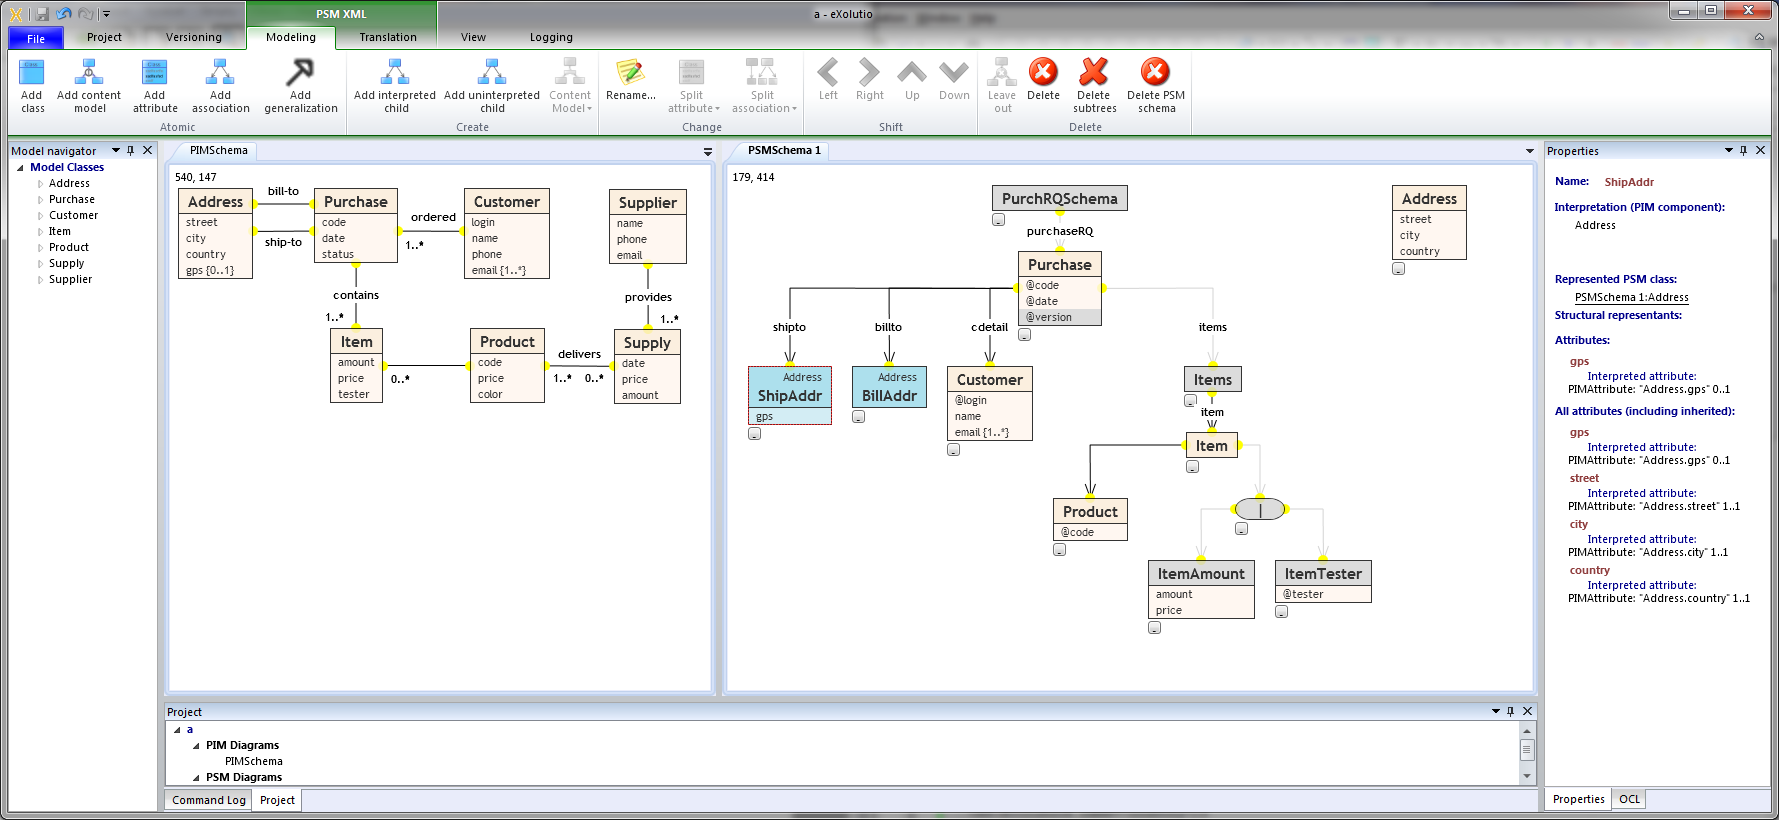
\includegraphics[width=0.8\textwidth]{img/exolutio.png}
    \caption{Preview of the eXolutio tool. Left panel shows PIM model as UML class digram, whether the right panel represents a PSM schema in a tree-like structure, that can be converted to XML schema.}
\end{figure}

\section{Similar work}

Google Scholar docela něco vrací na "model driven transformation cim pim data schema". Dále pak jsem našel možná relevantní - https://link.springer.com/article/10.1007/s10270-021-00905-x. K článkům byste se měl z univerzitní sítě dostat zdarma.